\subsubsection{C-DAS}\label{subsubsec:c-das-litteraturstudie}
%Att som järnvägsföretag använda informationssystem för att minimera energikonsumtion och öka punktlighet blir alltmer utbrett~\cite{Bae2014, Kamenicky2016, Konstantinos2013, Cwil2018, Tschirner2013, Yang2013, Joborn2023}.
%Informationssystemet i fråga kallas C-DAS och står för \emph{driver advisory system}~\cite{Bae2014, Kamenicky2016, Konstantinos2013, Cwil2018, Tschirner2013, Yang2013, Joborn2023}.
\paragraph{}
\hspace{-11pt}
Att som järnvägsföretag använda informationssystem för att minimera energikonsumtion och öka punktlighet blir alltmer utbrett i Europa~\cite{Bae2014, Kamenicky2016, Konstantinos2013, Cwil2018, Tschirner2013, Yang2013, Joborn2023}.
Digitala förarverktyg kallas DAS (driver advisory system) och avser applikationer som ämnar stödja lokförare i deras yrkesutövande genom att bidra med hastighetsrekommendationer och situationsmedvetenhetsstöd på ett förtroendefullt sätt.
Det främsta syftet med DAS är dock att understödja lokförare i att ankomma i tid till stationer med minskad energikonsumtion~\cite{IRS90940}.
Ett DAS-system beräknar en rekommenderad körprofil utifrån erhållna parametrar, exempelvis tidtabell för tåget, befintlig hastighet och GPS-position och verkar oberoende av andra aktörer och system~\cite{IRS90940}.
%En lämplig strategi är att implementera ett connected driver advisory system (C-DAS)~\cite{Angel2020, Joborn2023, Lindmark2022, Ketech2022, Verstappen2022}.
DAS-system som inte har en koppling till infrastrukturförvaltarens kapacitetsstyrningssystem kallas S-DAS~\cite{IRS90940, Joborn2023, Angel2020, Olsson2023}.
S-DAS-system kan vara avancerade och sofistikerade i sig, det som särskiljer dem från C-DAS är avsaknaden av direktlänk till tågklarerare~\cite{IRS90940, Joborn2023, Angel2020, Olsson2023}.
Den här typen av system är vanliga i Sverige idag~\cite{Systemdefinition2019}.
DAS-system som istället har en direkt koppling mellan TMS och C-DAS-OB kallas C-DAS och står för \emph{connected driver advisory system}~\cite{Bae2014, Kamenicky2016, Konstantinos2013, Cwil2018, Tschirner2013, Yang2013, Joborn2023}.
Dessa informationssystem kan ta emot nya tidtabeller för tåget de körs på och beräknar således körprofil utifrån uppdaterade tidtabeller erhållna direkt från tågklarerare~\cite{Bae2014, Kamenicky2016, Konstantinos2013, Cwil2018, Tschirner2013, Yang2013, Joborn2023}.
Ett grafisk användargränssnitt med hastighetsrekommendationer och annan relevant information presenteras för lokförare genom en applikation i en surfplatta eller via inbyggd skärm i förarhyttens instrumentpanel~\cite{Bae2014, Kamenicky2016, Konstantinos2013, Cwil2018, Tschirner2013, Yang2013, Joborn2023, Lindmark2022, Angel2020}.
Idag finns flera implementerade digitala förarverktyg men de har sina begränsningar~\cite{Bae2014}.
Ofta omfattas inte kommunikation med tågklarerare eller TMS, eller så tas inte tillräcklig hänsyn till lokförarnas informationsbehov eller situationsmedvetenhet i beaktande~\cite{Bae2014, Joborn2023, Tschirner2013}.
\paragraph{}
\hspace{-11pt}
Ett protokoll har tagits fram av UIC\footnote{Union Internationale des Chemins de fer (Internationella järnvägsunionen)} specifikt för att standardisera digital kommunikation mellan tågtrafikledningssystem och lokförare i en C-DAS-kontext~\cite{Joborn2023, Olsson2023, Lindmark2022}.
%UIC, som verkar för att underlätta internationell järnvägstrafik, har tagit fram SFERA-standarden för detta ändamål.
Standarden benämns \emph{SFERA}, och skapades för att underlätta och främja internationell och gränsöverskridande järnvägstrafik\cite{IRS90940}.
%Genom att ta fram och ge ut normer för t.~ex.~hur järnvägsfordon ska karaktäriseras gynnar man trafik mellan olika länder.
Protokollet definieras i dokumentet UIC IRS 90940 som förutom att ge en bakgrund till systemet och dess syfte även beskriver datameddelandens uppsättning i XML-format~\cite{Joborn2023, IRS90940}.
%I det definieras hur datautbytet ska se ut mellan TMS och C-DAS-ombordenhet, dvs standardiserad digital kommunikation mellan tågklarerare och lokförare.
Ett system som tillämpar denna standard skulle möjliggöra för tågklarerarna att direkt kunna kommunicera med lokförarna genom datameddelanden och därmed tilldela tågen nya tidtabeller i ett operativt läge~\cite{Angel2020, Joborn2023, Lindmark2022, Olsson2023}.
%Protokollet definieras som XML-schema~\cite{Olsson2023}.
\subsubsection{TMS}
Ett system för att operativt planera och styra järnvägstrafik kallas \emph{traffic management system} (TMS)~\cite{Joborn2023}.
Styrningssystemet Digital graf/STEG som utvecklas, används och förvaltas av Trafikverket är ett exempel.
Användarna är av detta system är främst Trafikverkets tågklarerare.
När en avvikelse eller trafikstörning uppstår kan en tågklarerare digitalt justera tågs överskådliga tidtabell för att optimera hålltider.
Det kan till exempel vara att vid enkelspårsdrift anpassa två mötande tågs tidtabeller så att de kan passera varandra på en mötesstation \emph{utan} att behöva stanna att och \emph{utan} att tappa tid.
Detta trots att den ursprungliga tidtabellen kanske medger att ett av tågen ska hålla en högre hastighet fram till mötesstationen och sedan invänta sitt mötande tåg.
En förutsättning är att något eller båda tågens tidtabeller innehåller effektiviseringsutrymme som tillåter lägre hastighet utan att tåget blir försenat~\cite{Joborn2023}.
Trafikverkets C-DAS-pilotprojekt som skedde på Malmbanan och i samarbete med godstågsföretaget Kaunis Iron visade exempelvis att väl time:ade tågmöten hade god effekt på energiförbrukningen~\cite{Lindmark2022}.
På detta vis möjliggörs körning som är skonsammare och mer hållbar för både fordon och bana; inbromsning till stopp och acceleration tillbaka till marschfart kan exempelvis utebli för ett eller båda tåg till förmån för effektuttag.
Körning i med farthållning kan annars innebära acceleration i motlut och inbromsning i medlut vilket leder till omotiverad energiförbrukning~\cite{Lindmark2022}.
Att exempelvis som tungt lastat godståg stanna \lq{}i onödan\rq{} i brant motlut skulle också medföra en umbärlig energiförbrukning~\cite{Lindmark2022}.
Istället kan C-DAS-ombordsystemet rekommendera frirullning, planera för en jämnare acceleration eller föreslå en lägre hastighet utifrån det data som förses från TMS för föraren~\cite{Lindmark2022}.
Digital graf är ännu inte fullt utrullat hos Trafikverket; systemet är fortfarande i ett utvecklingsstadium~\cite{Joborn2023}.
\paragraph{}
\hspace{-11pt}För att den nya uppdaterade körplanen ska kunna verkställas måste den som tidigare nämnt delges föraren på tåget vars körplan förändrades via ett gränssnitt.
Det nuvarande systemet som används i Sverige för operativ planering och ämnas ersättas av Digital graf/STEG saknar stöd för att varken ta emot digital information från lokföraren, justera tidtabeller digitalt i realtid eller digitalt delge tåg uppdaterad körprofil~\cite{Systemdefinition2019, Joborn2023}.
Nya grafer (grafiska representationer av tidtabeller) ritas istället för hand med penna och papper, och informationen delges föraren muntligen via GSM-R-telefonsamtal.
C-DAS-konceptet omsluter istället hela kedjan av kommunikation från tågklarerarens omplanerade tidtabeller för tåg, till TMS datadistributionssystem, till berörd C-DAS-server, till C-DAS-ombordenhet, till förare tillbaka med bekräftelse från förare till tågklarerare att information mottagits~\cite{IRS90940}.
En förutsättning för att dessa anpassningar ska kunna verkställas utan att något tåg tappar tid och blir försenat är förekomsten av s.k. \emph{slack} i tidtabellen.
Slack betyder att ett tåg inte behöver hålla sin STH för att vara i tid till nästa uppehåll - med eller utan trafikutbyte (resenärer på/av)~\cite{Lindmark2022}.
% TODO: !!
%Man går från proaktiv planering till proaktiv + reaktiv planering etc~\cite{IRS90940}.
\subsubsection{Dataflödet inom C-DAS enligt SFERA}
När tågklarerare utför omplanering av tidtabeller sker detta i det TMS infrastrukturförvaltaren har implementerat.
När en omplanering är gjord tolkas informationen av en server som skickar vidare informationen till berört järnvägsföretages server.
Infrastrukturförvaltarens och järnvägsföretagets server kallas enligt SFERA IM DAS-TS respektive RU DAS-TS\cite{Joborn2023, IRS90940}.
RU DAS-TS prenumererar på det data som förses av IM DAS-TS och när ny information emottagits vidarebefordras den till berört tåg och lokförare.
RU DAS-TS kan även på förhand förse IM DAS-TS med information rörande tågets statiska förutsättningar såsom tåglängd, tågvikt, dynamisk vikt, typ av fordon, STH\footnote{Största tillåtna hastighet. Tågsättets STH är den lägsta av följande hastigheter: \emph{drivfordonets} största tillåtna hastighet (om det finns någon särskild begränsning för den aktuella sträckan enligt uppgift i linjeboken), största tillåtna hastighet för det långsammaste fordonet, tillåten hastighet för den aktuella sträckan med hänsyn till tågsättets bromsförmåga enligt reglerna i TTJ-modul 11 (broms), tillåten hastighet med hänsyn till tågsättets axellast, tillåten hastighet med hänsyn till begränsningar i förarens utbildning, hastighet enligt säkerhetsorder om hastighetnedsättning utan signalering~\cite{TTJ2015}.}, motoreffekt (hk), bromskraft och så vidare~\cite{IRS90940}.
Lokföraren tar emot informationen via en applikation ombord på tåget som benämns C-DAS-OB~\cite{Joborn2023, IRS90940}\@.
Denna applikation räknar i slutändan ut en rekommenderad hastighetsprofil baserat på flera olika datapunkter och begränsande faktorer~\cite{Joborn2023, Olsson2023}.
Om körprofilen som räknas ut av C-DAS-OB ryms inom den nya tidtabellen återges den för föraren som sedan följer den~\cite{IRS90940, Sfera-usecase-poster-2022}.
Om den beräknade körprofilen inte ryms inom den nya tidtabellen skickas ett automatiskt svar till tågklareraren som får agera därefter~\cite{Sfera-usecase-poster-2022}.
%En server-sida hos infrastrukturförvaltaren som tolkar tågklarerarens nya, uppdaterade, tidtabell för ett visst tåg och tillhandahåller detta för en server hos berört järnvägsföretag.
%Järnvägsföretagets server vidarebefordrar sedan datapaketet åt vederbörande klient ombord på ett tåg, som i sin tur beräknar en hastighetsprofil och återger för lokföraren~\cite{Yao2022, Olsson2023, Joborn2023, IRS90940}.
Järnvägsföretagets server vidarebefordrar sedan datapaketet åt vederbörande klient ombord på ett tåg, som i sin tur beräknar en hastighetsprofil och återger för lokföraren~\cite{Olsson2023, Joborn2023, IRS90940}.
%Beräkning kan även ske direkt på järnvägsföretagets server.
Se figur~\ref{fig:C-DAS-kommunikation} för visuell beskrivning av SFERA:s dataflödesmodell för C-DAS-kommunikation.
\begin{figure}[hbt!]
    \centering
    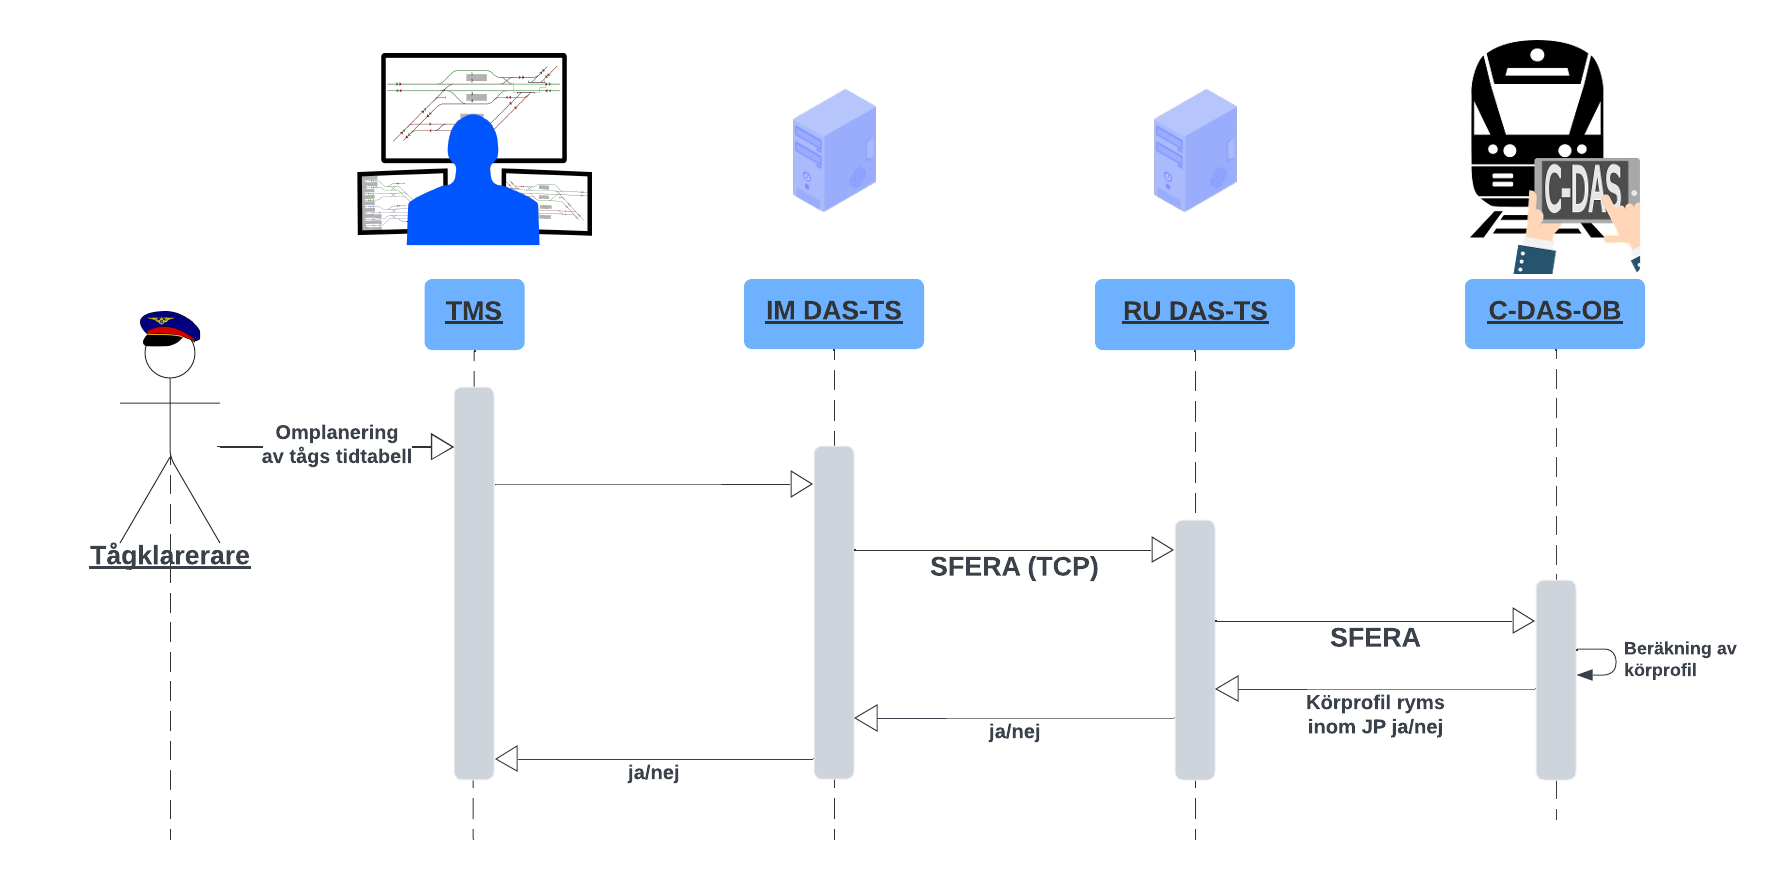
\includegraphics[width=0.8\textwidth]
    {c-das-comms}
    \caption{Sekvensdiagram som visar C-DAS dataflöde enligt SFERA-protokollet när en tågklarerare planerar om ett tågs tidtabell. Egen framställning/Wikimedia Commons Public Domain.}
    \label{fig:C-DAS-kommunikation}
\end{figure}
\paragraph{}
Möjligheterna med C-DAS är många:
\begin{itemize}
    \item Effektivare planering av operativ järnvägstrafik~\cite{Joborn2023}
    \item Ökad operativ precision i positionering av tåg~\cite{Systemdefinition2019}
    \item Förbättrad och förenklad kommunikation mellan tågklarerare och lokförare~\cite{Systemdefinition2019}
    \item Utökad kapacitet, utan att behöva genomföra (ofta dyra) infrastrukturprojekt~\cite{Ketech2022, Lindmark2022, Olsson2023, Verstappen2022}
    \item Förbättrad hantering vid trafikstörningar~\cite{Angel2020, Joborn2023, Lindmark2022, Systemdefinition2019, Ketech2022, Verstappen2022}
    \item Förbättrad punktlighet vid trafikstörningar~\cite{Angel2020, Joborn2023, Lindmark2022, Systemdefinition2019, Ketech2022, Verstappen2022}
    \item Reducerat effektuttag från järnvägsinfrastrukturens kraftförsörjningssystem~\cite{Angel2020, Joborn2023, Lindmark2022, Systemdefinition2019, Ketech2022, Olsson2023, Verstappen2022}
    \item Reducerat slitage på infrastruktur~\cite{Angel2020, Joborn2023, Lindmark2022, Systemdefinition2019, Ketech2022, Olsson2023}
    \item Minskat slitage på järnvägsfordon (bromssystem, hjul m.m.)~\cite{Angel2020, Joborn2023, Systemdefinition2019, Ketech2022, Lindmark2022, Olsson2023}
    \item Minskade verksamhetskostnader för järnvägsföretag till följ av minskat slitage och energikonsumtion~\cite{Ketech2022}
    \item Ökad trafiksäkerhet till följd av lägre hastigheter samt färre antal restriktiva signaler och stoppsignaler ~\cite{Olsson2023}
    \item Förbättrad trafikinformation till järnvägsföretagens kunder~\cite{Angel2020, Ketech2022, Lindmark2022}
    \item Förbättrat beslutsstöd för tågklarerare~\cite{Lindmark2022, Ketech2022}
    \item Gemensam lägesbild mellan lokförare och tågklarerare~\cite{Lindmark2022, Ketech2022}
    \item Bättre komfort för resenärer~\cite{Lindmark2022, Systemdefinition2019}
    \item Förbättrad arbetsmiljö för (främst) tågklarerare, lokförare och annan ombordpersonal~\cite{Systemdefinition2019}
    \item Minskad miljöpåverkan~\cite{Lindmark2022}
    \item Harmoniserat trafikflöde~\cite{Systemdefinition2019}
\end{itemize}

Om inte en tågklarerare kan jobba i ett digitalt planeringsverktyg kan inte C-DAS användas som en lösning för att förbättra trafikflöden och spara tid, energi och pengar~\cite{Tschirner2013}.
För att minska arbetsbelastningen för tågklarerare det därför viktigt att alla systemets delar integreras väl i deras digitala miljö för att minimera arbetsbelastning~\cite{Tschirner2013, Joborn2023}.
Att behöva göra regelbundna byten mellan fönster och applikationer kan försämra arbetsmiljön och göra att de glömmer information~\cite{Tschirner2013, Lindmark2022}.
Systemet behöver hjälpa tågklarerare att identifiera störningar och sedan hantera dem~\cite{Tschirner2013, Joborn2023}.
En tågklarerares arbete måste och göras tillgängligt för så många intressenter som möjligt, i synnerhet lokförare och andra tågklarerare, och när en tidtabell uppdateras måste det omedelbart kommuniceras till berörd(a) lokförare~\cite{Tschirner2013}.
När omplaneringar görs enligt SFERA distribueras den nya tidtabellen till berörd lokförare ut och C-DAS-OB räknar därefter ut om det går att skapa en körprofil som respekterar tidtabellens ramar~\cite{Sfera-usecase-poster-2022}.
Om detta inte går skickas ett meddelande automatiskt till tågklarerare att den nya tidtabellen (journey profile) inte kan respekteras~\cite{Sfera-usecase-poster-2022} och det blir upp till TC att fatta nya beslut.
Att en C-DAS/TMS-lösning omfattar informationsflöde åt båda hållen, dvs.~både från tågklarerare till lokförare samt vice versa är således av stor vikt~\cite{Tschirner2013}.
Utan dessa förutsättningar kan allt arbete med C-DAS göras obsolet~\cite{Tschirner2013}.

CATO:
~\cite{Yang2013,Lindmark2022,Tschirner2013}
\paragraph{}
\hspace{-11pt}
Slutsatsen som kan dras av det som publicerats i forskningsforum och bland Trafikverkets interna dokument gör gällande att DAS-applikationer, deras tillämpning och dess algoritmer har studerats väl.
I forskningen läggs stor vikt vid algoritmer och beräkning av körprofil men inte kommunikation ur lokförarens perspektiv.
Kommunikationsprotokollet SFERA har inte granskats och utvärderats i någon publicerad vetenskaplig forskning.

\subsubsection{Gamification}

Litteraturstudie av dessa artiklar redovisas med ingående under~\ref{subsec:dokumentanalys} som del av studiens datainsamling.